\documentclass[]{article}
\usepackage{lmodern}
\usepackage{amssymb,amsmath}
\usepackage{ifxetex,ifluatex}
\usepackage{fixltx2e} % provides \textsubscript
\ifnum 0\ifxetex 1\fi\ifluatex 1\fi=0 % if pdftex
  \usepackage[T1]{fontenc}
  \usepackage[utf8]{inputenc}
\else % if luatex or xelatex
  \ifxetex
    \usepackage{mathspec}
  \else
    \usepackage{fontspec}
  \fi
  \defaultfontfeatures{Ligatures=TeX,Scale=MatchLowercase}
\fi
% use upquote if available, for straight quotes in verbatim environments
\IfFileExists{upquote.sty}{\usepackage{upquote}}{}
% use microtype if available
\IfFileExists{microtype.sty}{%
\usepackage{microtype}
\UseMicrotypeSet[protrusion]{basicmath} % disable protrusion for tt fonts
}{}
\usepackage[margin=1in]{geometry}
\usepackage{hyperref}
\hypersetup{unicode=true,
            pdftitle={Drugs and Jobs: The effect of unemployment on drug overdose deaths in America},
            pdfauthor={Evan Arnold and Caleb Ren},
            pdfborder={0 0 0},
            breaklinks=true}
\urlstyle{same}  % don't use monospace font for urls
\usepackage{graphicx,grffile}
\makeatletter
\def\maxwidth{\ifdim\Gin@nat@width>\linewidth\linewidth\else\Gin@nat@width\fi}
\def\maxheight{\ifdim\Gin@nat@height>\textheight\textheight\else\Gin@nat@height\fi}
\makeatother
% Scale images if necessary, so that they will not overflow the page
% margins by default, and it is still possible to overwrite the defaults
% using explicit options in \includegraphics[width, height, ...]{}
\setkeys{Gin}{width=\maxwidth,height=\maxheight,keepaspectratio}
\IfFileExists{parskip.sty}{%
\usepackage{parskip}
}{% else
\setlength{\parindent}{0pt}
\setlength{\parskip}{6pt plus 2pt minus 1pt}
}
\setlength{\emergencystretch}{3em}  % prevent overfull lines
\providecommand{\tightlist}{%
  \setlength{\itemsep}{0pt}\setlength{\parskip}{0pt}}
\setcounter{secnumdepth}{0}
% Redefines (sub)paragraphs to behave more like sections
\ifx\paragraph\undefined\else
\let\oldparagraph\paragraph
\renewcommand{\paragraph}[1]{\oldparagraph{#1}\mbox{}}
\fi
\ifx\subparagraph\undefined\else
\let\oldsubparagraph\subparagraph
\renewcommand{\subparagraph}[1]{\oldsubparagraph{#1}\mbox{}}
\fi

%%% Use protect on footnotes to avoid problems with footnotes in titles
\let\rmarkdownfootnote\footnote%
\def\footnote{\protect\rmarkdownfootnote}

%%% Change title format to be more compact
\usepackage{titling}

% Create subtitle command for use in maketitle
\newcommand{\subtitle}[1]{
  \posttitle{
    \begin{center}\large#1\end{center}
    }
}

\setlength{\droptitle}{-2em}

  \title{Drugs and Jobs: The effect of unemployment on drug overdose deaths in
America}
    \pretitle{\vspace{\droptitle}\centering\huge}
  \posttitle{\par}
    \author{Evan Arnold and Caleb Ren}
    \preauthor{\centering\large\emph}
  \postauthor{\par}
      \predate{\centering\large\emph}
  \postdate{\par}
    \date{12/06/2019}


\begin{document}
\maketitle

\section{Introduction and Motivation}

Overdose deaths in the US have increased dramatically since 1999. Opioid
use deaths in particular have reached epidemic levels, with a 200\%
increase in overdose deaths between 2000 and 2014 (Ghertner and Groves
2018). The Centers for Disease Control and Prevention estimates that
over 60,000 drug overdose deaths occurred in 2016, three times the rate
of drug deaths as 1999 (Hedegaard and Warner 2018)

\section{Exploratory Data Anslysis Methods}

\subsection{Data Summary}

As a next step in our project, we collected data from the CDC in the
form of the Vital Statistics Rapid Release dataset (VSRR). The VSRR data
contains provisional counts of drug overdose deaths in the US as
reported by agencies from all 50 states and the District of Columbia.
The data is collected on a monthly basis.

The data of import to this project is the number of deaths in each state
as a result of drug overdose. Drug overdoses are counted by state
agencies in acordance to World Health Organization standards, which lay
out the basic guides for reporting agencies to code and classify causes
of death. Drug categories that are represented in this dataset include
the major drivers of the opioid epidemic like heroin (coded by T40.1),
natural opioid analgesics (morphine and codeine), synthetic opioids
(oxycodone, hydrocodone, oxymorphone; T40.2), methadone (T40.3), other
synthetics (fentanyl, tramadol; T40.4) and other drugs like cocaine,
methamphetamine, etc.

There were over 26052 data points from the VSRR dataset. Of those data
points, many are individual observation of different coded deaths from
different drugs; after reshaping and data cleaning, there are now 2652
individual observations. The data ranges from Januart 1, 2015 to April
1, 2019, with each state reporting 52 observations (once per month).
Overdose deaths range from 55 deaths in the month of May 2015 in South
Dakota to a high of 5697 in Pennsylvania in September of 2017.

Unemployment data was sourced from the Bureau of Labor Statistics.
Unemployment data is published in monthly increments from the Bureau of
Labor Statistics by state. Data is published beginning in 1976 and is
published on the first of each month describing the previous month's
unemployment rate.

There is a very specific definition of who in the labor force is
considered \emph{unemployed}. According to the BLS, those who are
currently unemployed are those who are ``jobless, looking for a job, and
avaiable for work.'' People who are incarcerated, in a nursing home, or
in a mental health care facility are not considered unemployed as they
are not fit for work.

Using this definition, data was scraped from the BLS website and
aggregated by each state and the District of Columbia. The unemployment
rate in percent is given by the \texttt{unemployment} column. The lowest
unemployment rate in a given state and month is Vermont in 2019 with a
2.1\% unemployment rate. The highest rate is DC in 2015 with a 7.4\%
unemployment rate. The data itself is roughly Normally distributed with
a mean of 4.2\% and a median of 4.31\%.

Here we consider a series of variables from the Federal Reserve Bank of
St.~Louis (Federal Reserve Economic Data or FRED for short). All such
datasets are originally from Bureau of Labor Statistics or the U.S.
Census Bureau, however, FRED has their data in a more convenient format.

First, we consider the number of new private housing units authorized by
building permit. This timeseries is reported monthly. In our analysis,
this variable serves as a proxy to housing development as well as the
health of the housing market; more permits implies a healthy housing
market and ample housing options. We thus expect a negative association
between overdose deaths and new housing permits.

Next, we consider the money spent on imports of manufactored and
non-manufactored commodities in millions of dollars. This timeseries is
reported monthly. This feature will offer our analysis an insight into
the health of the state-local manufactoring sector. In the past few
years, the states with some of the worst opioid overdose numbers are
those in in the Rust Belt
(\url{https://www.drugabuse.gov/drugs-abuse/opioids/opioid-summaries-by-state}).
One potential narrative is that the increased use of overseas labor
stips entire communities of their jobs, and many of those effected turn
to opioids. We can reasonably quantify this effect by state with the
number of dollars spent on imports. We expect an increase in spending on
imports to imply a decrease in availability of manufactoring jobs and
the health of the local manufactoring sector, and thus we expect a
positive association between import spending and overdose deaths.

Now, we consider the value of manufactored and non-manufactored exports
in millions of dollars. This timeseries is reported monthly. We hope to
use this variable as another perspective on the health of manufactoring
and the availability of jobs in the manufactoring sector. We expect the
value of exports to have a negative association with overdose deaths.

Finally, we consider per capita personal income in dollars. This
timeseries is reported annually. It is reasonable to assume that the
average personal income does not change dramatically intrayear. Per
capita income affords us a glimpse into the personal financial freedom
of state residents. We chose to include per capita income instead of
median household income in order to capture the influence of the
wealthly. We expect a negative association between income and overdose
deaths.

Below, we include annual population estimates from the Census Bureau. We
use annual data for two reasons: the availability of state population
estimates is limited and we can reasonably assume that state population
does not change dramatically intrayear. Furthermore, we use the
population estimate from the previous year as a given year's population
variable. We do so becuase population estimates are generated late into
the year, and thus for any given year, the previous year's Census Bureau
estimate is likely more accurate. We will use population to normalize
the other predictors.

R inherently has several statistics about states. Most of these are
static estimates from the early 70's (population estimates, income per
capita, illiteracy,\ldots{}). We can, however, use the datasets which
give information about the region a state is in. This is a categorical
variable with four categories: northeast, northcentral, south, and west.
Though the nomenclature is dated, these categories reasonably divide
states by potentially important factors. For example, we expect the Rust
Belt (which R includes in the region northcentral) to have a positive
association with overdose deaths (as noted above). Here we note that we
have to encode Washington DC ourselves as the data in R does not contain
the District of Columbia (in accordance with R's encoding, Washington DC
is in the south).

R also provides us with the area of each state in square miles. Again,
we must encode Washington DC manually (Fogle 2019).

Before we begin any modeling or analyis, we must normalize overdose
deaths, permits, imports, and exports. By doing so, we convert each to a
rate which can be directly compared across states. In order to avoid
working with very small numbers, we convert each rate to: overdose
deaths per 100000 people, permits per 100000 people, spending on imports
in millions of dollars per 100000 people, and value of exports in
millions of dollars per 100000 people.

\subsection{EDA}

Below we check to see if any cells of the dataframe are NA, NULL, NaN,
or infinite. No such values exist. We have a relatively clean dataset.

\begin{verbatim}
## [1] FALSE
\end{verbatim}

We now consider the possibility of multicollinearity. As shown below,
some of the quantitative features of our dataset are highly correlated
(population and imports, imports and exports,\ldots{}). In order to
handle this multicolinearity, we will consider ensemble models such as
random forests.

\begin{verbatim}
##              unemployment     permits     imports     exports      income
## unemployment   1.00000000 -0.19668769  0.09159131  0.14169833 -0.08702747
## permits       -0.19668769  1.00000000 -0.08778809  0.10420801 -0.05360477
## imports        0.09159131 -0.08778809  1.00000000  0.44711152  0.07188101
## exports        0.14169833  0.10420801  0.44711152  1.00000000 -0.02178304
## income        -0.08702747 -0.05360477  0.07188101 -0.02178304  1.00000000
## population     0.15069205 -0.02456117  0.43294469  0.19201412  0.12074508
## area           0.25436018  0.02988105 -0.13252477  0.19145599 -0.04051548
##               population        area
## unemployment  0.15069205  0.25436018
## permits      -0.02456117  0.02988105
## imports       0.43294469 -0.13252477
## exports       0.19201412  0.19145599
## income        0.12074508 -0.04051548
## population    1.00000000  0.14993987
## area          0.14993987  1.00000000
\end{verbatim}

\begin{center}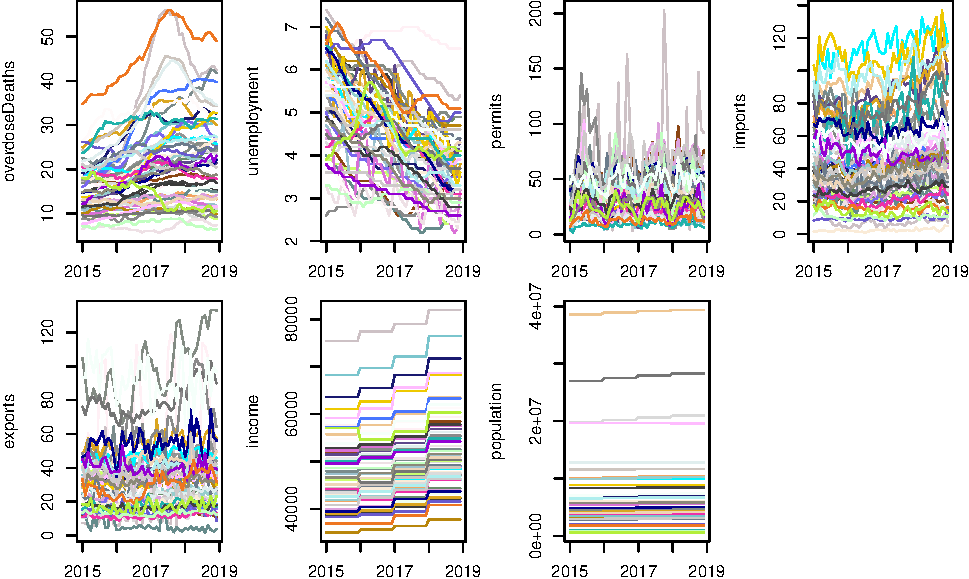
\includegraphics{stat139_project_final_files/figure-latex/toy-1} \end{center}

\begin{center}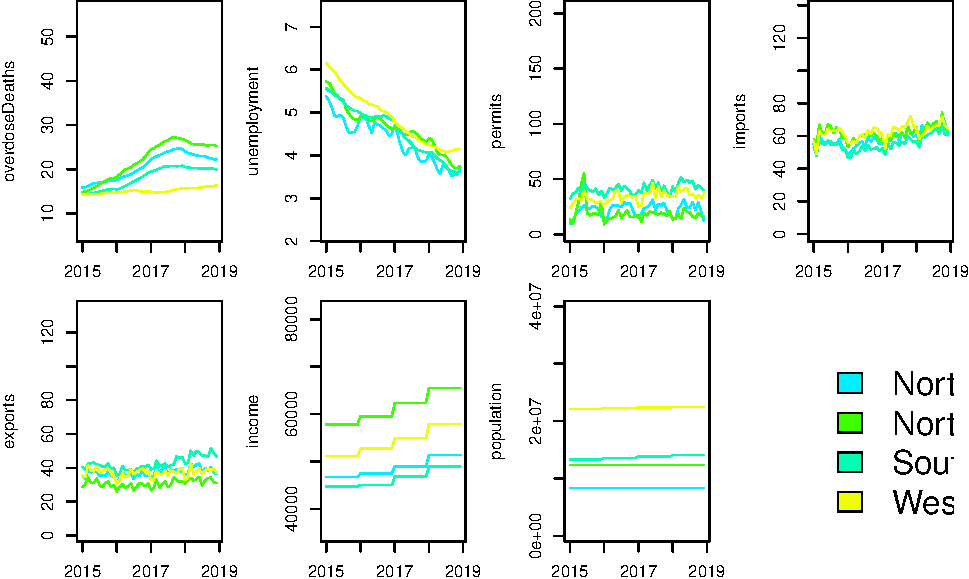
\includegraphics{stat139_project_final_files/figure-latex/toy-2} \end{center}

\begin{center}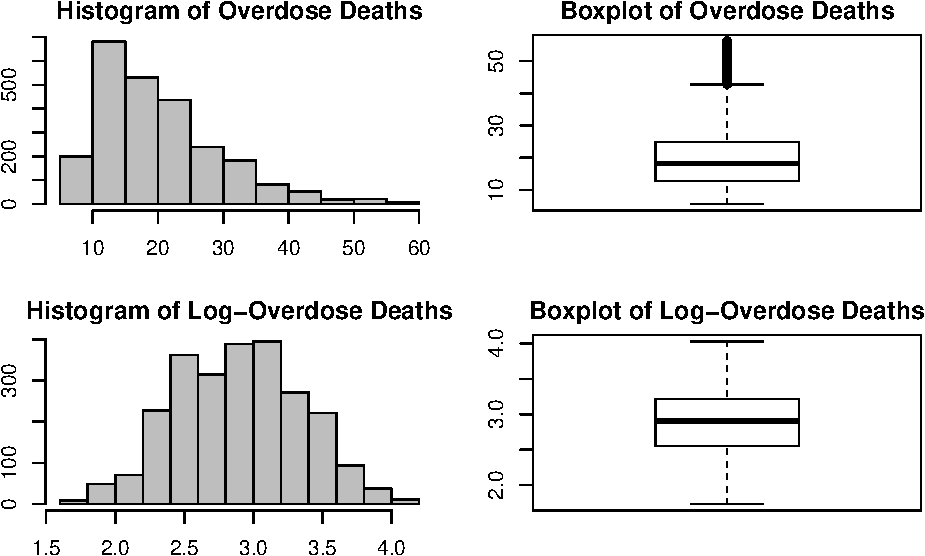
\includegraphics{stat139_project_final_files/figure-latex/unnamed-chunk-1-1} \end{center}

We see that the data is much closer to a Normal distribution if we apply
a log transformation. We shall predict the log-rate of overdose deaths
in our linear models.

\begin{center}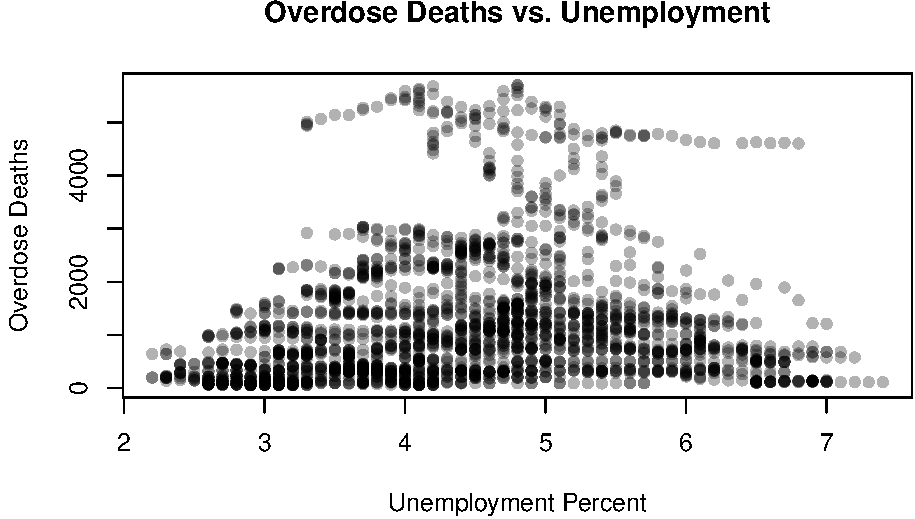
\includegraphics{stat139_project_final_files/figure-latex/unnamed-chunk-2-1} \end{center}

\section{Results}

\begin{verbatim}
## 
## Call:
## lm(formula = log(overdoseDeaths) ~ unemployment, data = train)
## 
## Residuals:
##      Min       1Q   Median       3Q      Max 
## -1.02505 -0.35466 -0.00048  0.31178  1.07295 
## 
## Coefficients:
##              Estimate Std. Error t value Pr(>|t|)    
## (Intercept)  2.504656   0.041741  60.004   <2e-16 ***
## unemployment 0.087923   0.009148   9.611   <2e-16 ***
## ---
## Signif. codes:  0 '***' 0.001 '**' 0.01 '*' 0.05 '.' 0.1 ' ' 1
## 
## Residual standard error: 0.4384 on 1936 degrees of freedom
## Multiple R-squared:  0.04554,    Adjusted R-squared:  0.04505 
## F-statistic: 92.37 on 1 and 1936 DF,  p-value: < 2.2e-16
\end{verbatim}

The simple regression model has a positive coefficient for unemployment
(\(0.09179\)). With a \(t\)-statistic of \(10.11\) (\(p\)-value
\(\approx 0\)), this coefficient is very significant. The model has a
positive association between unemployment and overdose deaths.

\begin{center}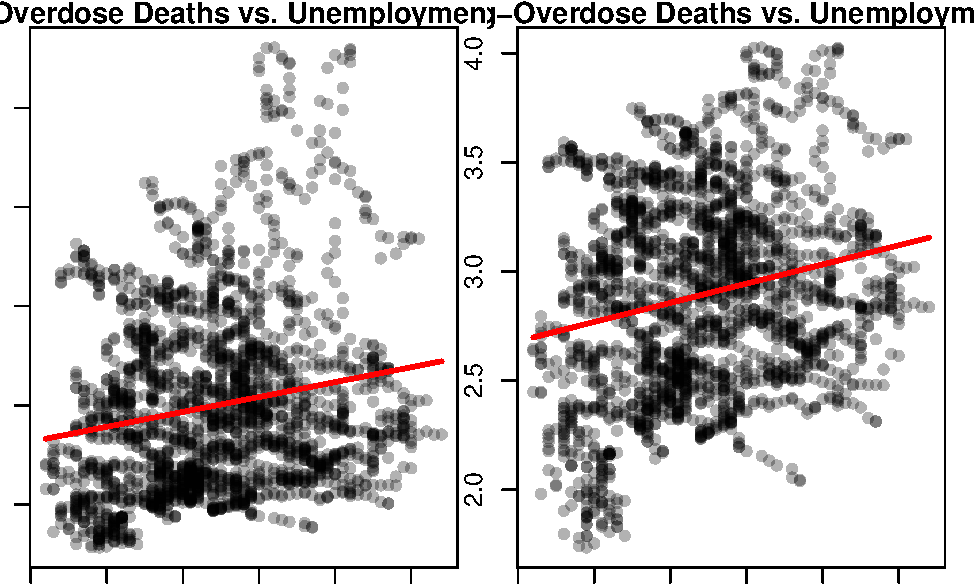
\includegraphics{stat139_project_final_files/figure-latex/unnamed-chunk-4-1} \end{center}

In order to better evaluate the importance of unemployment, we apply an
ESS F-test. First we fit two linear models. The first model include all
main effects except unemployment, while the second includes all main
effects. Then, we fit two quadratic models. The first model contains all
main effects and their respective quadratic variants except
unemployment. The second model contains the same predictors, except that
it includes unemployment and its quadratic effect. We again verify the
assumptions of a linear model via a plot of residuals vs.~fitten values.

\begin{verbatim}
## Analysis of Variance Table
## 
## Model 1: log(overdoseDeaths) ~ state + month + year + permits + imports + 
##     exports + income + population + region + area
## Model 2: log(overdoseDeaths) ~ state + month + year + permits + imports + 
##     exports + income + population + region + area + unemployment
##   Res.Df    RSS Df Sum of Sq      F    Pr(>F)    
## 1   1870 26.899                                  
## 2   1869 26.405  1   0.49353 34.933 4.047e-09 ***
## ---
## Signif. codes:  0 '***' 0.001 '**' 0.01 '*' 0.05 '.' 0.1 ' ' 1
\end{verbatim}

With an F-statistic of \(13.387\) (with \(1887\), \(1\) degrees of
freedom) and a corresponding p-value \(<0.001\), unemployment provides
significant predictive ability. We now consider the same ESS F-test with
quadratic models.

\begin{verbatim}
## Analysis of Variance Table
## 
## Model 1: log(overdoseDeaths) ~ state + month + year + poly(permits, 2, 
##     raw = T) + poly(imports, 2, raw = T) + poly(exports, 2, raw = T) + 
##     poly(income, 2, raw = T) + poly(population, 2, raw = T) + 
##     region + area
## Model 2: log(overdoseDeaths) ~ state + month + year + poly(permits, 2, 
##     raw = T) + poly(imports, 2, raw = T) + poly(exports, 2, raw = T) + 
##     poly(income, 2, raw = T) + poly(population, 2, raw = T) + 
##     region + area + poly(unemployment, 2, raw = T)
##   Res.Df    RSS Df Sum of Sq      F    Pr(>F)    
## 1   1865 25.280                                  
## 2   1863 24.347  2   0.93256 35.678 6.229e-16 ***
## ---
## Signif. codes:  0 '***' 0.001 '**' 0.01 '*' 0.05 '.' 0.1 ' ' 1
\end{verbatim}

\begin{center}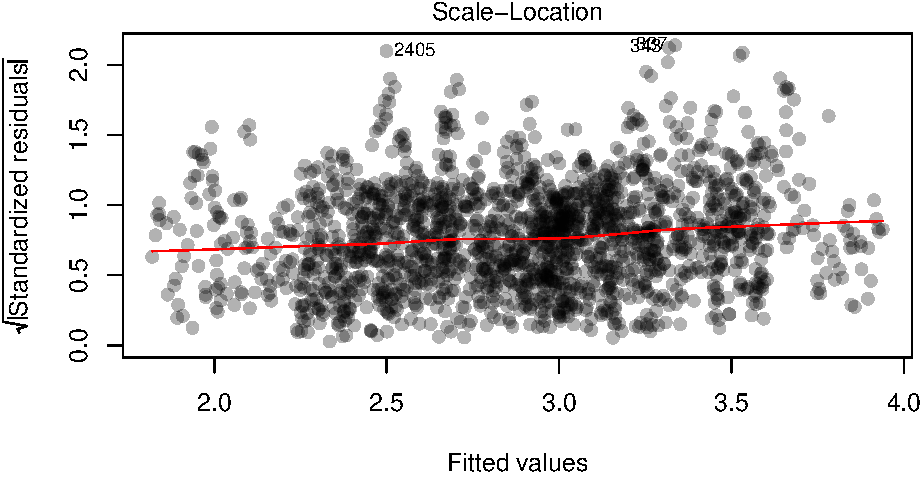
\includegraphics{stat139_project_final_files/figure-latex/polynomial-1} \end{center}

With an F-statistic of \(17.359\) (with \(1881\), \(2\) degrees of
freedom) and a corresponding p-value \(<0.001\), unemployment provides
significant predictive ability. Additionally, there seems to be no
underlying structure to the residuals, the residuals appear to have
reasonably constant variance, and are reasonably normally distributed:
the assumptions of our models (linearity, homoscedasticity of residuals,
and normality) appear to be satisfied.

In order to be thorough, we examine the importance of unemployment in
two additional ways: lasso regression, and random forrest regression. We
begin with lasso regression. Due to l1 penalty of lasso regression, less
important variables quickly converge to zero as the regularization
parameter increases. Below, we fit a lasso model (with the same dedign
matrix as that of the full quadratic kitchen sink model) with a series
of possible regularization parameters. We then consider the order in
which the variable coefficients shrink to zero.

\begin{center}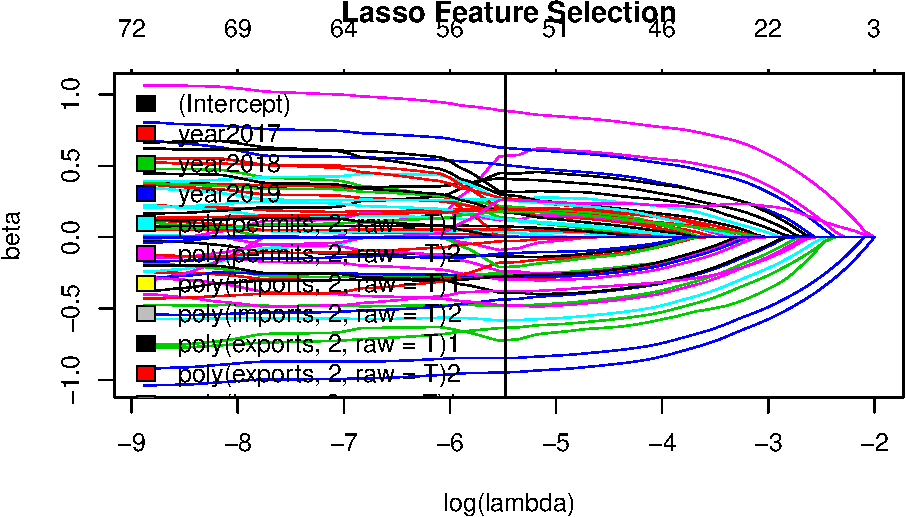
\includegraphics{stat139_project_final_files/figure-latex/lasso-1} \end{center}

Lasso feature selection agrees with the results of the ESS F-test.
Unemployment (the quadratic effect in this case) is one of the last
coefficients to shrink to zero along with population. We further test
this conclusion with a random forest model. Below, we fit a random
forest model with all main effects and then examine it's relative
feature importance.

\begin{center}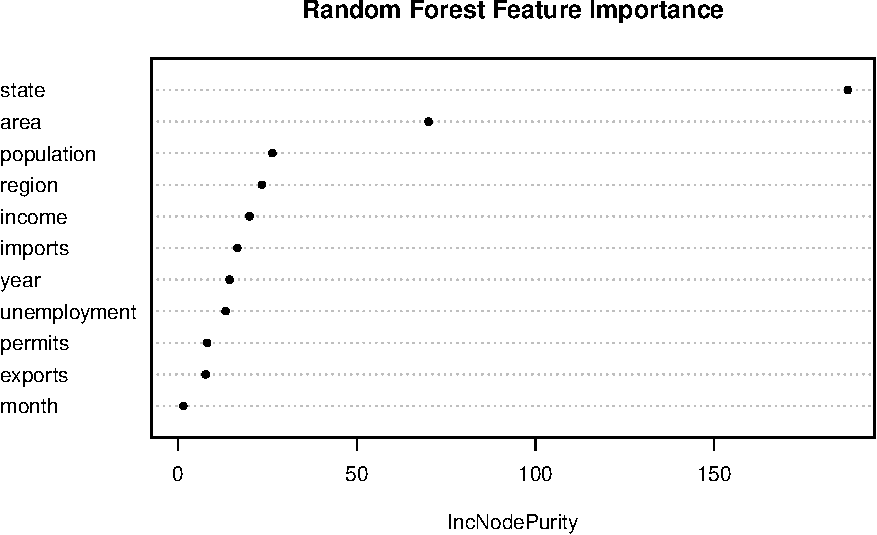
\includegraphics{stat139_project_final_files/figure-latex/rf-1} \end{center}

Unemployment is relatively not important in the random forest model. It
appears as though state and area (which is correlated with state) are
the most important predictors. In order to handle the grouped nature of
time, state, area, and so forth, we fit a mixed effects model.

Below, we fit a three-layered mixed-effects model. The first two layers
are state and year respectively. Theoretically, we would prefer to fit a
four-layered model which includes month below year. This is impossible
with our dataset (\(n = 2448\)). With 51 states, 5 years, and 12 months,
we would need a minimum of \(51 \times 5 \times 12 = 3060\) samples in
order to fit such am model. We include a random intercept for states and
years. The only random effect we include in the model is unemployment.
These are purposeful design choices considering the limited size of our
dataset. More complex models would not be reasonably fit.

\begin{verbatim}
##            train       test
## lm1   0.43816409 0.42957134
## lm2   0.11781197 0.12232569
## lm3   0.11672618 0.12119689
## poly1 0.11421185 0.11852647
## poly2 0.11208546 0.11606524
## lasso 0.11860396 0.12170799
## rf1   0.04815521 0.04625506
## lmer1 0.03287450 0.03876381
\end{verbatim}

\begin{center}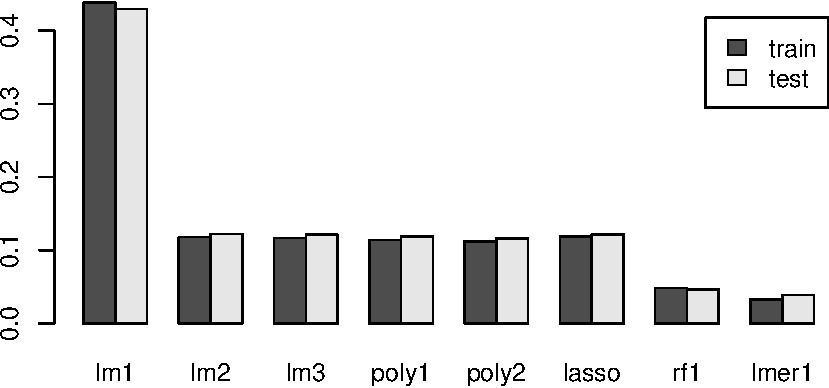
\includegraphics{stat139_project_final_files/figure-latex/rmse-1} \end{center}

\section{Conclusions and Decisions}

Based on root-mean-square error, the model that performs the best in
terms of minimizing predictive error on the holdout set would be the
random forest model.

\section{Direction of Future Research}

```

\section{References}

\hypertarget{refs}{}
\hypertarget{ref-Brittanica}{}
Fogle, J. M. 2019. \emph{Washington, D.C.} Encyclopaedia Brittanica.

\hypertarget{ref-Ghertner2018}{}
Ghertner, R., and L. Groves. 2018. ``The Opioid Crisis and Economic
Opportunity: Geographic and Economic Trends.'' \emph{Office of the
Assistant Secretary for Planning and Execution} 24 (September).

\hypertarget{ref-Hedegaard2018}{}
Hedegaard, A. M., H. M.D. Miniño, and M. Ph.D. Warner. 2018. ``Drug
Overdose Deaths in the United STates, 1999 - 2017.'' \emph{Centers for
Disease Control and Prevention} 329 (November).


\end{document}
